\documentclass[a4paper]{article}
\usepackage[utf8]{inputenc}
\usepackage{graphicx}
\usepackage[cm]{fullpage}
\usepackage{upgreek}
\usepackage{siunitx}
\usepackage{bm}
\usepackage{amsmath}
\usepackage{amsfonts}
\usepackage[colorinlistoftodos,prependcaption,textsize=tiny]{todonotes}
\newcommand{\A}{{\mathbb{A}}}
\newcommand{\K}{{\mathbb{K}}}
\newcommand{\J}{{\mathbb{J}}}
\newcommand{\G}{{\mathbb{G}}}
\newcommand{\Z}{{\mathbb{Z}}}
\newcommand{\C}{{\mathbb{C}}}
\newcommand{\W}{{\mathbb{W}}}
\newcommand{\R}{{\mathbb{R}}}
\newcommand{\M}{{\mathbb{M}}}
\newcommand{\N}{{\mathbb{N}}}
\newcommand{\LLL}{{\mathbb{L}}}
\newcommand{\SSS}{{\mathbb{S}}}
\newcommand{\HH}{{\mathbb{H}}}
\usepackage[maxnames=6]{biblatex}
\addbibresource{biblio.bib}
\newcommand{\bN}{{\mathcal{N}}}
\usepackage{hyperref}
\hypersetup{
colorlinks,
citecolor=black,
filecolor=black,
linkcolor=black,
urlcolor=black}


%%%%%%%%%%%%%%%%%%%%%%%%%%%%%%%%%%%%%%%%%%%%%%%%%%%%%%%%%%%
%%%%%%%%%%%%%%%%%%%%%%%%%%%%%%%%%%%%%%%%%%%%%%%%%%%%%%%%%%%
%%%%%%%%%%%%%%%%%%%%%%%%%%%%%%%%%%%%%%%%%%%%%%%%%%%%%%%%%%%

\title{FCUBED}
\author{C. Thieulot, A. Maitre, F. Gueydan}

\begin{document}
\maketitle
\tableofcontents

\textcite{grfr03}

\newpage
%%%%%%%%%%%%%%%%%%%%%%%%%%%%%%
\section{Physics \& Equations}

\subsection{Basic equations}


%-------------------------
\subsubsection{Stokes flow}

\begin{eqnarray}
\vec\nabla \cdot \bm \sigma + \rho \vec{g} &=& \vec{0} \\
\vec\nabla \cdot \vec\upnu &=& 0
\end{eqnarray}

\[
\bm\sigma = -p {\bm 1} +  \bm \tau
\]
\[
\bm\tau = 2 \eta \dot{\bm \varepsilon}(\vec\upnu)
\]

\begin{eqnarray}
-\vec\nabla p + \vec\nabla \cdot (2 \eta \dot{\bm \varepsilon}(\vec\upnu)) + \rho \vec{g} &=& \vec{0} \\
\vec\nabla \cdot \vec\upnu &=& 0
\end{eqnarray}

\[
\eta_{dsl} = \frac{1}{2} A^{-1/n} \dot\varepsilon_e^{1/n-1} 
\exp \frac{Q }{nRT}
\]
where $\dot\varepsilon_e$ is the effective strain rate defined as 
\[
\dot\varepsilon_e = \sqrt{\frac12 (
\dot\varepsilon_{xx}^2+
\dot\varepsilon_{yy}^2)+
\dot\varepsilon_{xy}^2
)} 
\]

\todo[inline]{describe plasticity}

\[
\sigma_y = p \sin\phi + c \cos \phi
\]


%-------------------------
\subsubsection{Darcy flow}

Following chapter 10 of Guy Simpson's book \textcite{simp17} 
the equations governing the evolution of the fluid pressure and 
fluid flow velocities are\footnote{I have slightly 
changed the notations.}
\begin{eqnarray}
\varphi \beta \frac{\partial p_f}{\partial t} &=& -\vec\nabla \cdot \vec \upnu + H -\frac{\partial \varphi}{\partial t}\label{eq:128:a}\\
\vec\upnu &=& -\frac{K}{\eta_f} \vec\nabla p_f \label{eq:128:b}
\end{eqnarray}
\todo[inline]{is this the equation we want to use ? other ref ? what are other ppl using ?}

where
\begin{itemize}
\item $p_f$ is the pore fluid pressure,
\item $\vec\upnu$ is the fluid velocity vector,
\item $\varphi$ is the porosity\footnote{\url{https://en.wikipedia.org/wiki/Porosity}} (-). 
Wikipedia: ``Porosity or void fraction is a measure of the void (i.e. "empty") spaces 
in a material, and is a fraction of the volume of voids over the total volume, 
between 0 and 1, or as a percentage between 0\% and 100\%''. 

\item $\beta$ is the bulk compressibility\todo{typical values for rocks?} (\si{\per\pascal}),
\todo[inline]{we find online multiple compressbilities in the context of rocks. Which are we to use?}

\item $K$ is the permeability\footnote{\url{https://en.wikipedia.org/wiki/Permeability_(Earth_sciences)}} (\si{\square\meter})
Wikipedia: ``
Permeability is a property of porous materials that is an indication of the ability for fluids (gas or liquid) to flow through them. Fluids can more easily flow through a material with high permeability than one with low permeability. The permeability of a medium is related to the porosity, but also to the shapes of the pores in the medium and their level of connectedness. Fluid flows can also be influenced in different lithological settings by brittle deformation of rocks in fault zones; the mechanisms by which this occurs are the subject of fault zone hydrogeology. Permeability is also affected by the pressure inside a material.''

In the code it is assumed to be given by \textcite{skre16,begu18}
\[
K = K_0 \left( \frac{\phi}{\phi_0}  \right)^3
\]
where $K_0$ is the permeability at a reference porosity $\phi_0$.

\item $\eta_f$ is the fluid viscosity (\si{\pascal\second}), typically water\footnote{\url{https://en.wikipedia.org/wiki/Water}}
\item $\rho_f$ is the water density (\si{\kg\per\cubic\meter}),
\item $g$ is acceleration due to gravity (\si{\meter\per\square\second}),
\item $\vec{e}$ is a unit vector oriented in the vertical direction,
\item $H$ accounts for any fluid pressure sources or sinks (e.g., due to devolatilization reactions)
\end{itemize}
substituting \eqref{eq:128:b} into \eqref{eq:128:a} lead to a single parabolic equation for
the excess fluid pressure as follows:
\begin{equation}
\varphi \beta  \frac{\partial p_f}{\partial t}
=
\vec\nabla \cdot \left( \frac{K}{\eta_f} \vec\nabla p_f  \right) + H
-\frac{\partial \phi}{\partial t}
\end{equation}
Note that once the excess pressure is computed one can recover the fluid velocity via
$\vec\upnu=-\frac{K}{\eta_f} \vec\nabla p_f$.
Note that $H=0$ in experiments 1,2,3.

\todo[inline]{}


In what follows we assume the buoyancy forces are negligible, i.e. 
the term $\rho \vec{g}$ is neglected.


\subsubsection{Coupling}

Remark1: 
when using tectonic dt (which is ${\cal{O}}(10^5)$ year, 
we find that $\frac{\partial \phi}{\partial t}
\simeq \frac{\phi^n -\phi^{n-1}}{\delta t } \rightarrow 0$
so that the contribution of this term to the equation is 
virtually inexistant.

Remark2: Likewise the characteristic Darcy time is probably 
about ${\cal{O}}(10^0)$ year so that when carrying out 
tectonic time steps the Darcy diffusion process has the time 
to reach steady state. Since we are currently not
relying on an operator splitting approach, we might as well
directly solve the steady state Darcy equation, i.e.
$\partial p_f/\partial t \rightarrow 0$. 




\newpage
%%%%%%%%%%%%%%%%%%%%%%%%%%%%%%
\section{Numerical aspects}

2D

Cartesian domain

Finite elements

quadrilateral elements Q2Q1

solver

%-------------------------------------------
\subsection{FE formulation of the equations}


\subsubsection{Stokes equations}


\subsubsection{Darcy equations}
Applying standard FE methodology to what is essentially a diffusion equation, we arrive at:
\[
{\M} \cdot {\vec{\dot{\cal{P}}}}_e  + {\K}_d \cdot \vec{\cal P}_e = rhs
\]
with
\[
{\M} = \int_\Omega \varphi \beta \vec{\bN}^T \vec{\bN} 
\]
\[
\K_d = \int_\Omega {\bm B}^T {\bm B} \frac{K}{\eta_f} 
\]
\[
rhs = \int_\Omega \vec\bN^T  H 
\]
Using a simple first order time discretisation yields
\[
({\M} + {\K}_d \delta t) \cdot \vec{\cal P}_e^n = \M \cdot \vec{\cal P}_e^{n-1} + rhs \delta t
\]



%..................................
\subsection{Specific algorithms}

%..................................
\subsubsection{computing time step}

CFL dt

%..................................
\subsubsection{Generating weak seeds}

Poisson disc distribution
seeds generated in square.
Notes that seeds which are kept are those inside circle or size ainclusion-w

For each marker $im$ we test whether it is at a distance of $w$ or less of 
seed $is$ and the prescribed strain is then parameterised as follows
\[
A \frac{1}{2} \left(\cos (\pi \frac{\sqrt{(x_{im}-x_{is})^2+(y_{im}-y_{is})^2}}{w}) +1 \right)
\]
where $w$ is the radius of the seed, and $A$ its maximum amplitude


\todo[inline]{include image examples}


%..................................
\subsubsection{Time dependent b.c.}

At the moment these are parameterised by $t_1$, $t_2$ and velofact.

\begin{verbatim}
       +-----------------+ -- velofact
       |                 |
-------|-----------------|------> time
       t1                t2
\end{verbatim}



%..................................
\subsubsection{Nonlinear residual}



%---------------------------------------------------
\subsection{Numerical parameter values and meaning}


\subsubsection{Marker in cell technique}

projection/averaging , advection, periodic pc, painting



...

\newpage
%%%%%%%%%%%%%%%%%%%%%%%%%%%%%%
\section{Benchmarks}

\subsection{Pure shear}

\subsection{Simple shear}

%-----------------
\subsection{SolVi}

\begin{center}
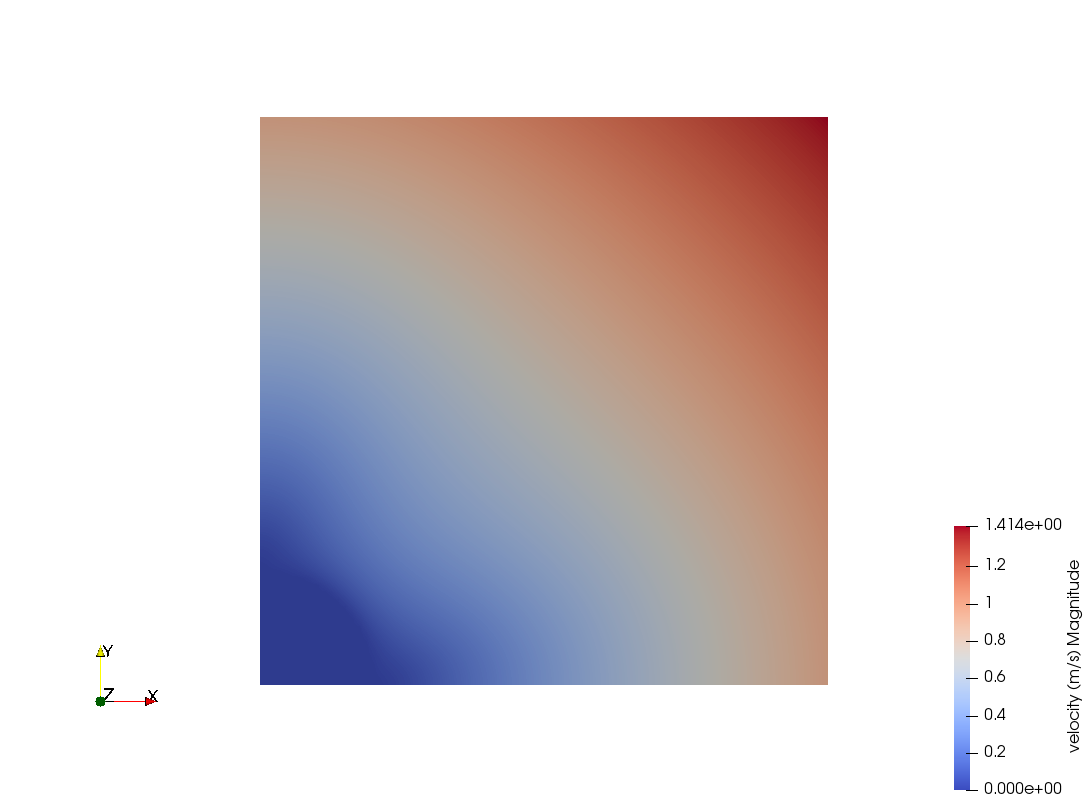
\includegraphics[width=8cm]{./results/benchmark_solvi/vel}
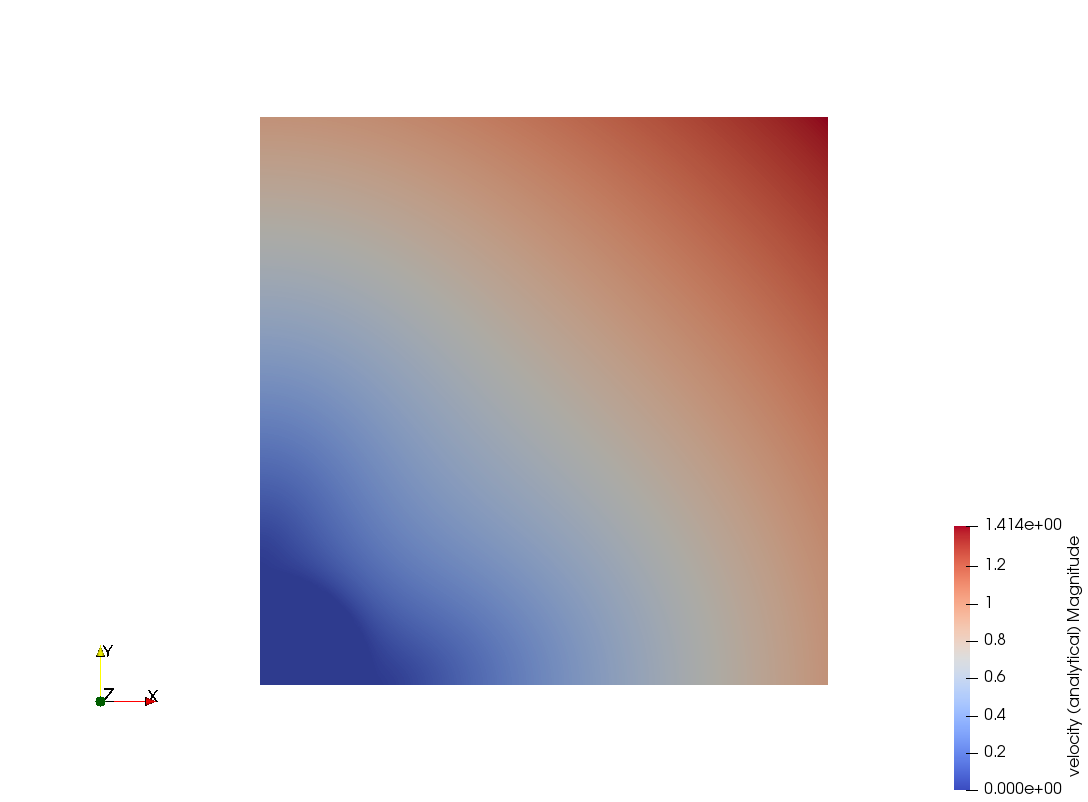
\includegraphics[width=8cm]{./results/benchmark_solvi/vel_analytical}\\
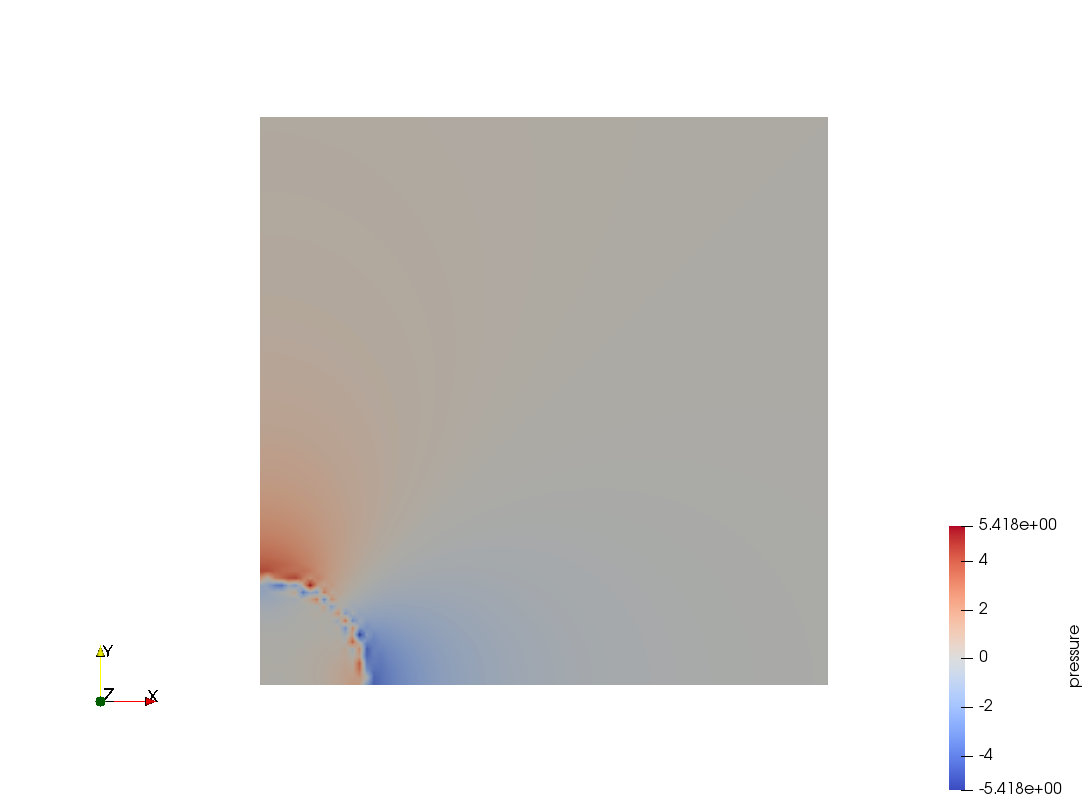
\includegraphics[width=8cm]{./results/benchmark_solvi/press}
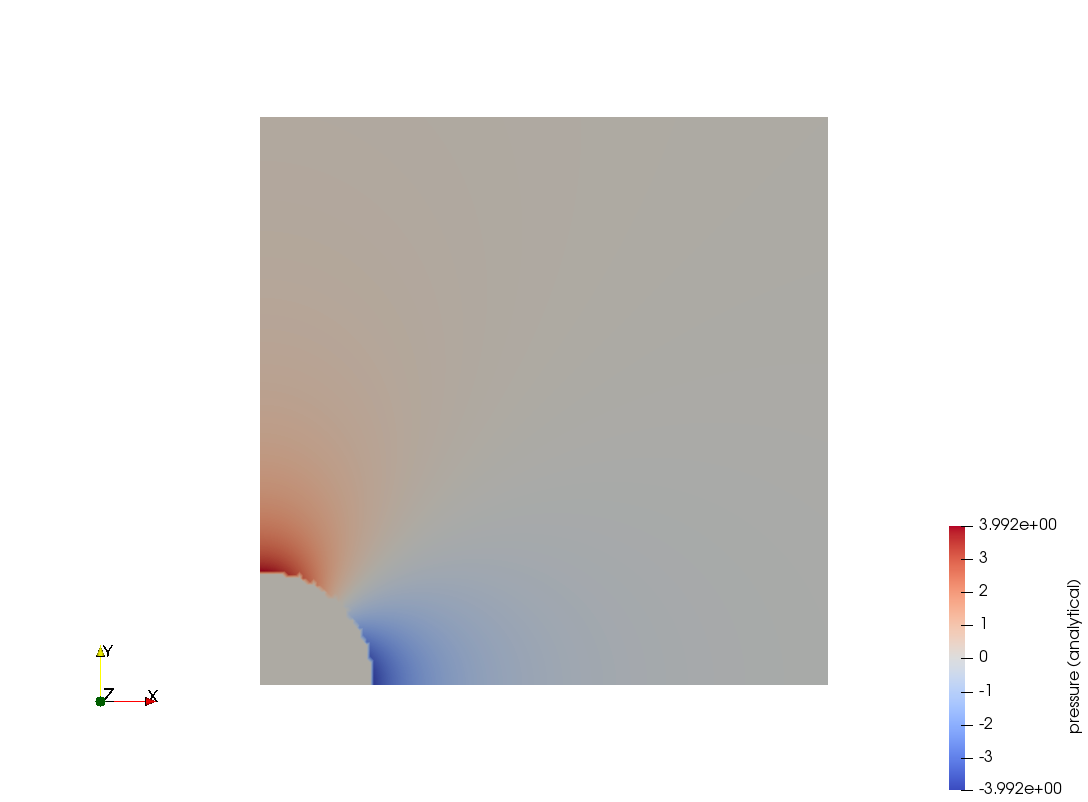
\includegraphics[width=8cm]{./results/benchmark_solvi/press_analytical}
\end{center}

\begin{center}
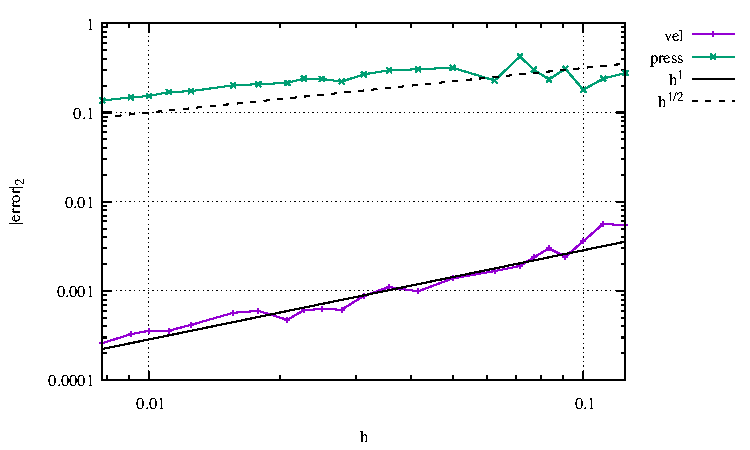
\includegraphics[width=8cm]{./results/benchmark_solvi/convergence.pdf}
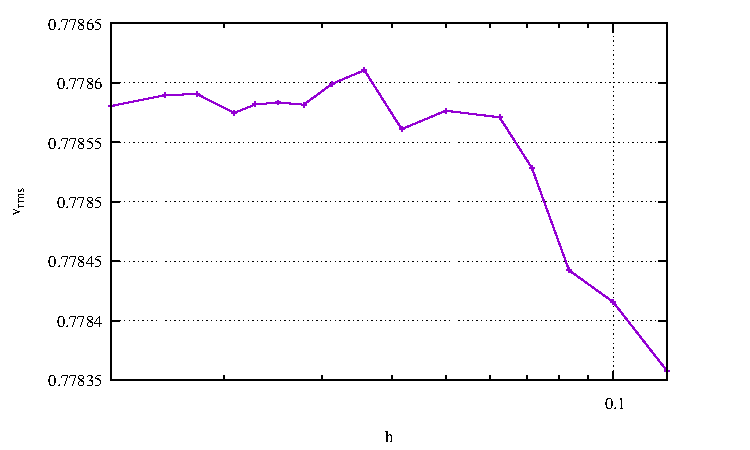
\includegraphics[width=8cm]{./results/benchmark_solvi/vrms.pdf}
\end{center}



\subsection{Poiseuille nonlinear}

\subsection{(E)VP experiment gerya 3 mats}

\subsection{darcy? simpson ?}

\subsection{gaussian diffusion in time}






%%%%%%%%%%%%%%%%%%%%%%%%%%%%%%
\newpage
\printbibliography
\end{document}


